\chapter{Árbol de Derivación}
\textbf{Definición: }Sea $G=\{\Sigma_N,\Sigma_T,S,P\}$ una gramática libre de contexto(GLC). Un AD es un árbol ordenado, construido recursivamente como sigue:
\begin{enumerate}
\item Un árbol sin aristas cuyo único vértice tiene etiqueta $S$, es un AD de $S$.
\item Si $x\in \Sigma_N$ es etiqueta de una hoja $h$ de un AD $A$, entonces:
	\begin{itemize}
	\item Si $x\rightarrow \varepsilon \in P$, entonces el árbol obtenido incrementando a $A$ un vértice $v$ con etiqueta $\varepsilon$ y una arista $\{h,v\}$ es un AD.
	\item Si $x\rightarrow x_1x_2...x_n \in P$, donde $x_1,x_2,...x_n \in \Sigma_T \cup \Sigma_N$, entonces el árbol obtenido incrementando a $A$ $n$ vértices $v_1,v_2,...,v_n$ con etiquetas $x_1,x_2,...,x_n$ en ese orden, y con $n$ aristas $\{h,v_1\},\{h,v_2\},...\{h,v_n\}$ es un AD. 
	\end{itemize}
\end{enumerate}

\textbf{Ejemplo: }Sea $G$ un GLC donde $P$ está dado por:
\begin{align*}
& E\rightarrow E+T|T	\\
& T\rightarrow T+F|F	\\
& F\rightarrow (E)|t
\end{align*}
Obtener el AD para la cadena $w=t+(t+t)$, partiendo de E.

\textbf{Solución: }
\begin{align*}
E	&\rightarrow T			&\qquad (R_2)\\
	&\rightarrow T+F		&\qquad (R_3)\\
	&\rightarrow T+(E)		&\qquad (R_5)\\
	&\rightarrow T+(E+T)	&\qquad (R_1)\\
	&\rightarrow T+(T+T)	&\qquad (R_2)\\
\intertext{Luego se aplica las reglas reiteradas veces, uno a la vez}
	&\rightarrow F+(T+T)	&\qquad (R_4)\\
	&\rightarrow F+(F+T)	&\qquad (R_4)\\
	&\rightarrow F+(F+F)	&\qquad (R_4)\\
	&\rightarrow t+(F+F)	&\qquad (R_6)\\
	&\rightarrow t+(t+F)	&\qquad (R_6)\\
	&\rightarrow t+(t+t)	&\qquad (R_6)
\end{align*}
%GRAFICO 1
\begin{figure}[h!]
\centering
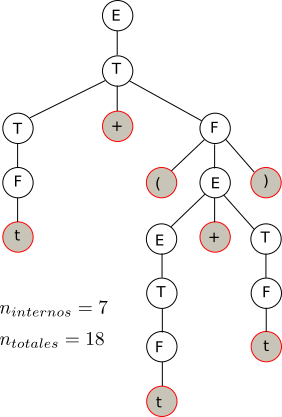
\includegraphics[width=0.3\textwidth]{img_15_1.png}
\caption{Arbol de derivación}\label{img_15_1}
\end{figure}
Se ha requerido 11 pasos para derivar $w$ (Fig \ref{img_15_1}).

Cada nodo interno del árbol será un símbolo no terminal, mientras que las hojas serán los símbolos terminales. Una regla $A:= x_1...x_n$ se representará como un símbolo cuyo nodo padre es A, siendo sus nodos hijos $x_1,x_2,...,x_n$.

\textbf{Ejemplo: }Sea $G$ la GLC dada por:
\begin{align*}
S	&\rightarrow AB		& \\
	&\rightarrow aA|a	& \\
	&\rightarrow bB|b	& \\
\intertext{Obtener el Árbol de Derivación para $w=aabbb$ e indicar la cantidad de pasos}
\intertext{\textbf{Solución: }}
S	&\rightarrow AB		&(R_1)	\\
	&\rightarrow aAB	&(R_2)	\\
	&\rightarrow aaB	&(R_3)	\\
	&\rightarrow aabB	&(R_4)	\\
	&\rightarrow aabb	&(R_5)	\\
\end{align*}
%GRAFICO 2
\begin{figure}[h!]
\centering
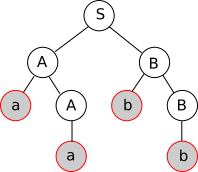
\includegraphics[width=0.22\textwidth]{img_15_2.png}
\caption{Arbol de derivación}\label{img_15_2}
\end{figure}
\begin{align*}
\left. \begin{array}{c}
n_i=4	\\
n_T=9
\end{array}\right \} \mbox{Pasos }=9-4=5 \quad \cmark
\end{align*}
\textbf{Definición: }Una GLC $G$ se llama ambigua, cuando es posible obtener dos o mas ADs diferentes para alguna sentencia que genere. Puede haber otras gramáticas GLC equivalente a una GLC ambigua, y que éstas gramáticas no sean ambiguas.

\textbf{Ejemplo: }Sea $G$ una GLC donde P esta dado por:
\begin{align*}
S	&\rightarrow S+S	&(R_1)	\\
	&\rightarrow S*S	&(R_2)	\\
	&\rightarrow (S)	&(R_3)	\\
	&\rightarrow t		&(R_4)	\\
\intertext{Obtener el AD para $w=t+t+t$ partiendo de $S$.}
\end{align*}
\textbf{Solución: }
\begin{align*}
S	&\rightarrow S+S	&(R_1)	\\
S	&\rightarrow S+S+S	&(R_1)	\\
S	&\rightarrow t+S+S	&(R_4)	\\
S	&\rightarrow t+t+S	&(R_4)	\\
S	&\rightarrow t+t+t	&(R_4)
\end{align*}
\begin{enumerate}
\item $n_i=5$, $n_t=10$.
%GRAFICO 3 
\begin{figure}[h!]
\centering
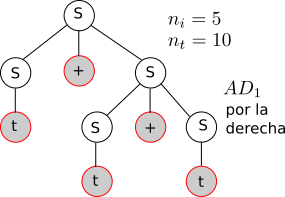
\includegraphics[width=0.3\textwidth]{img_15_3.png}
\caption{Arbol de derivación}\label{img_15_3}
\end{figure}
\item 
\begin{align*}
S	&\rightarrow S+S	&(R_1)	\\
S	&\rightarrow t+S	&(R_4)	\\
S	&\rightarrow t+S+S	&\mbox{ERROR }(R_1)	\\
S	&\rightarrow t+t+S	&(R_4)	\\
S	&\rightarrow t+t+t	&(R_4)
\end{align*}
%GRAFICO 4
\begin{figure}[h!]
\centering
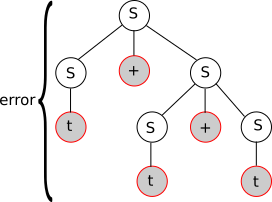
\includegraphics[width=0.45\textwidth]{img_15_4.png}
\caption{Arbol de derivación}\label{img_15_4}
\end{figure}

\begin{align*}
S	&\rightarrow S+S	&(R_1)	\\
S	&\rightarrow S+S+S	&(R_1)	\\
S	&\rightarrow S+S+t	&(R_4)	\\
S	&\rightarrow t+S+t	&(R_4)	\\
S	&\rightarrow t+t+t	&(R_4)
\end{align*}
%GRAFICO 5
\begin{figure}[h!]
\centering
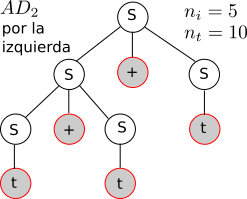
\includegraphics[width=0.45\textwidth]{img_15_5.png}
\caption{Arbol de derivación}\label{img_15_5}
\end{figure}

El (1) se puede interpretar como
$$\downlegend{t}{segundo}+(\underbrace{t+t}_{primero})$$
El (2) se puede interpretar como
$$(\underbrace{t+t}_{primero})+\downlegend{t}{segundo}$$
\end{enumerate}
\textbf{Definición: }Una derivación se denomina derivación a la izquierda si en cada paso, se expande la variable más a la izquierda.

Una derivación se dirá derivación a la derecha si en cada paso se expande la variable más a la derecha.

\textbf{Ejemplo: }Sea $G$ una GLC donde P está dado por:
\begin{align*}
S	&\rightarrow SbS	&(R_1)	\\
S	&\rightarrow ScS	&(R_2)	\\
S	&\rightarrow a		&(R_3)	\\
\end{align*}
Para la cadena $w=abaca$.
\begin{enumerate}
\item Obtener una derivación por la izquierda.
\item Obtener una derivación por la derecha.
\item Obtener su AD.
\end{enumerate}
\textbf{Solución: }
\begin{enumerate}
\item 
\begin{align*}
S	&\rightarrow \underline{S}bS	&(R_1)\\
	&\rightarrow ab\underline{S}	&(R_3)\\
	&\rightarrow ab\underline{S}cS	&(R_2)\\
	&\rightarrow abacS				&(R_3)\\
	&\rightarrow abaca				&(R_3)
\end{align*}
\item
\begin{align*}
S	&\rightarrow Sc\underline{S}	&(R_2)\\
	&\rightarrow \underline{S}ca	&(R_3)\\
	&\rightarrow Sb\underline{S}ca	&(R_1)\\
	&\rightarrow \underline{S}baca	&(R_3)\\
	&\rightarrow abaca				&(R_3)
\end{align*}
\item $\,$\\
%GRAFICO 6
\begin{figure}[h!]
\centering
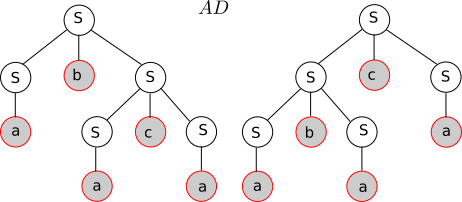
\includegraphics[width=0.4\textwidth]{img_15_6.png}
\caption{Arbol de derivación}\label{img_15_6}
\end{figure}
\end{enumerate}
\section{Equivalencia en Gramáticas}
Un mismo lenguaje puede ser generado por diversas gramáticas. Es recomendable simplificar estas gramáticas eliminando símbolos o reglas no deseadas.

\textbf{Definición: }Dos gramáticas $G^1$ y $G^2$ se llaman equivalentes, si ambas general el mismo lenguaje sobre $\Sigma_T$. Es decir:
$$L(G^1)=L(G^2)$$
\subsubsection{Elementos Indeseables en Gramáticas}
\textbf{Definición: }Una regla innecesaria es una producción de la forma $A:=A$.

\textbf{Definición: }Sea $G=(\Sigma_N,\Sigma_T,S,P)$ una GLC. Una variable $X\in \Sigma_N$ se llama útil si y solo si existen dos cadenas $u,v\in\Sigma^*$ tales que:
\begin{align*}
S	\xrightarrow{*} uXv \mbox{ y existe } w\in{\Sigma_T}^* \mbox{ tal que } uXv\xrightarrow{*}w
\end{align*}
\textbf{Definición: }Un símbolo inaccesible o inútil es aquel símbolo no terminal que no aparece en ninguna cadena de símbolos que pueda derivarse a partir del símbolo inicial de la gramática.

\textbf{Ejemplo: }Sea $G$ la GLC dado por:
\begin{align*}
S	&\rightarrow AB|a	\\
B	&\rightarrow b	\\
C	&\rightarrow c	\\
\intertext{Identifique las variables inútiles}
\end{align*}
\textbf{Solución: }
\begin{itemize}
\item C es una variable inútil. No existen subcadenas $u,v$ tales que $S\xrightarrow{*}uCv$.
\item A es inútil?. Vemos subcadenas $u,v$ tales que $S\rightarrow AB$, $u=\varepsilon,v=B$ pero $AB\xrightarrow{*}$?. No existe $w\in{\Sigma_T}^*$, luego A es inútil.
\item B es inútil, a pesar que.
\begin{align*}
S\rightarrow AB	\\
u=A	\\
v=\varepsilon\\
\intertext{No existe w tal que }
AB\xrightarrow{*} w
\end{align*}
\end{itemize}

\textbf{Definición: }Un símbolo no generativo es aquel símbolo no terminal a partir del cual no puede derivarse ninguna cadena de símbolos terminales.

Sea $G^1 =(\Sigma_N^1, \Sigma_T, S, P^1)$ una GLC. Transformaremos $G^1$ en $G^2=(\Sigma_N^2, \Sigma_T, S, P^2)$ de modo que $L(G^1)=L(G^2)$ y para todo $A\in\Sigma_N^2$ se obtenga $A\xrightarrow{*}w$ para algún $w\in\Sigma_T^*$.

\textbf{Algoritmo}
\begin{enumerate}
\item Inicializar $\Sigma_N^2$ con las variables $A$ tales que $A\rightarrow w$ es una regla de $G^1$ donde $w\in\Sigma_T^*$
\item Inicializar $P^2$ con todas las reglas $A\rightarrow w$ para los cuales $A\in \Sigma_N^2$ y $w\in\Sigma_T^*$.
\item $\;$\\
\begin{tabular}{p{4cm}p{8cm}}
Repetir:	&	\\
		&Añadir a $\Sigma_N^2$ todas las variables $A$ para los cuales $A\rightarrow w$ para algún $w\in(\Sigma_N^2\cup\Sigma_T)^*$ que sea una producción de $P^1$ y añadirla a $P^2$.	\\
Hasta que no se puedan añadir mas variables a $\Sigma_N^2$	&
\end{tabular}		
\end{enumerate}

\textbf{Ejemplo: }Sea la gramática $G^1$:
\begin{align*}
S	&\rightarrow Aa|B|D	\\
\cmark \; B	&\rightarrow b		\\
A	&\rightarrow aA|bA|B\\
\cmark \; C	&\rightarrow abd
\end{align*}
Use el algoritmo anterior, para obtener una gramática sin símbolos no generativos.
\textbf{Solución: }
\begin{align*}
\Sigma_T	&=\{a,b,d\}	\\
\Sigma_N^1	&=\{ S,A,B,C,D\}	\\
\end{align*}
\begin{enumerate}
\item $\Sigma_N^2=\{B,C\}$
\item $P^2: \left \{ \begin{array}{l}
B\rightarrow b	\\
C\rightarrow abd
\end{array}\right.$
\item $\Sigma_N^2=\{ B,C,S,A\}$
	\begin{enumerate}
	\item $\;$\\
	\begin{align*}
	&S\rightarrow B	&\;	\\
	&A\rightarrow B	&\;	\\
	&P^2:\left \{ \begin{array}{l}
		B \rightarrow b	\\
		C \rightarrow abd	\\
		S \rightarrow B	\\
		A \rightarrow B
	\end{array}\right.	&\;
	\end{align*}
	\item $\;$\\
	\begin{align*}
	&S \rightarrow Aa	&\;	\\
	&A \rightarrow aA	&\;	\\
	&A \rightarrow bA	&\;	\\
	&P^2:\left \{ \begin{array}{l}
		B \rightarrow b	\\
		C \rightarrow abd	\\
		S \rightarrow B|Aa
	\end{array}\right.	&\;
	\end{align*}
	\item $S \rightarrow D$. Donde $D$ no está en $\Sigma_N^2$
	\end{enumerate}
\end{enumerate}